\documentclass[11pt,final,hidelinks]{article}
\usepackage{lmodern}
\usepackage[T1]{fontenc}
\usepackage[english]{babel}
\usepackage[utf8]{inputenc}
\usepackage[activate={true,nocompatibility},final,tracking=true,kerning=true,
    spacing=true,factor=1100,stretch=10,shrink=10]{microtype}
\microtypecontext{spacing=nonfrench}
\usepackage[margin=1in]{geometry}
\usepackage{graphicx}
\graphicspath{{img/}}
\usepackage{caption}
\usepackage{subcaption}
\usepackage{booktabs}
\usepackage{array}
\usepackage{mathtools}
\usepackage{enumitem}
\usepackage{commath}
\usepackage{appendix}
\renewcommand\appendixtocname{Appendices}
\usepackage{amsmath}
\usepackage{amsthm}
\usepackage{amssymb}
\usepackage{pgfplots}
\usepackage{tikz}
\usepackage{tikzscale}
\usepackage[square,numbers]{natbib}
\bibliographystyle{plain}
\usepackage{siunitx}
\numberwithin{equation}{section}
\usepackage[hypertexnames=false]{hyperref}
\usepackage{cleveref}

\pgfplotsset{compat=newest}

\usepackage[fancy,section]{alex}

\hypersetup{
    pdftitle={Composition of Bernoulli sets},
    pdfauthor={Alexander Towell},
    pdfsubject={computer science},
    pdfkeywords={
        probabilistic data structure,
        approximate set,
        bloom filter,
        set operations,
        interval arithmetic,
        compositional algebra},
    colorlinks=true,
    linkcolor=magenta,
    citecolor=green,
    filecolor=blue,
    urlcolor=green
}

\title
{
    Composition of Bernoulli sets
}
\author
{
    Alexander Towell\\
    \texttt{atowell@siue.edu}
}
\date{2026}

\begin{document}
\maketitle
\begin{abstract}
Bernoulli sets---random approximate sets with independent, element-wise errors parameterized by false positive and false negative rates---are closed under set-theoretic composition.
We record closed-form error rates for complement, union, intersection, and set difference of independently constructed Bernoulli sets.
Each operation yields a (possibly higher-order) Bernoulli set: the per-element error probability depends on which operands contain the element, so the single false positive and false negative rate pair reported for the result is a cardinality-weighted marginal.
That pair is not sufficient input for further composition; nested expressions must carry the per-region rates.
The formulas are elementary consequences of independence and coincide with the independent-OR and independent-AND rules used for Bloom filters, combinational logic, and probabilistic databases; no novelty is claimed for them.
We also give subset and equality probabilities and an interval arithmetic treatment of uncertain rate parameters.
These results build on the Bernoulli set model introduced in a companion paper~\cite{bernoulliSets}, which establishes the axioms, error-count distributions, and asymptotic limits assumed here.
\end{abstract}

% Status and errata box (October 2026 freeze). \input right after \end{abstract}.
\begingroup
\setlength{\fboxsep}{7pt}%
\begin{center}
\fbox{\begin{minipage}{0.93\linewidth}\small
\setlength{\parskip}{4pt}%
\setlength{\parindent}{0pt}%
\textbf{Status and errata (October 2026).}
This is the final version of this preprint; no further revisions are planned.
It is superseded by Chapter~6 (\emph{Composition of Sets}), with the Boolean
groundwork in Chapter~3 (\emph{Boolean Algebra Under Noise}), of the monograph
\emph{Bernoulli Types: Two-Sided Error in Approximate Membership, Retrieval,
and Computation} (A.~Towell, 2026),
\url{https://metafunctor.com/latex/bernoulli-monograph/book.html}
(project hub: \url{https://metafunctor.com/research/bernoulli/}).
Please cite the monograph in preference to this preprint.

\textbf{Corrections in this version.}
\begin{itemize}\setlength{\itemsep}{1pt}\setlength{\parskip}{0pt}
\item Abstract, introduction, conclusion: a composed set's marginal (FPR, FNR) pair is not valid input for further composition; ``any set-theoretic expression'' now requires region-by-region application.
\item \Cref{sec:set_ops_summary}: new remark on nested expressions. Counterexample: in $(\tilde{A}_1 \cap \tilde{A}_2) \cup \tilde{A}_3$ at $\fprate = 0.02$, $\fnrate = 0.10$, two negatives have error $0.03764$ and $0.020392$.
\item \Cref{sec:set_theory}: cross-set independence is an added assumption (fails for reused operands, shared seeds); the monoidal fold of marginal pairs is exact only for the uniform rate.
\item \Cref{sec:set_theory}: a marginal rate averaging regions has a Poisson-binomial count. \Cref{sec:intervals}: bounds assume known partition weights.
\item \Cref{sec:relational}: the corollary for $\fprate = 0$ was mislabeled ``positive''; corrected, and the $\fnrate = 0$ case added.
\end{itemize}

\textbf{Predecessors credited.} The per-element channel is randomized
response~\cite{warner1965randomized}. The union and intersection rules are the
independent-OR and independent-AND rules of Bloom filter
analysis~\cite{bloom1970,broderMitzenmacher2004,papapetrou2010}, of signal
probability in combinational logic~\cite{parker1975,krishnaswamy2008ptm}, and of
probabilistic databases~\cite{dalvi2007}. No novelty is claimed for them.
A dated list of changes is in \texttt{ERRATA.md} in the source repository.
\end{minipage}}
\end{center}
\endgroup


\microtypesetup{protrusion=false}
\tableofcontents
\microtypesetup{protrusion=true}

%%%%%%%%%%%%%%%%%%%%%%%%%%%%%%%%
% Introduction
%%%%%%%%%%%%%%%%%%%%%%%%%%%%%%%%

\section{Introduction}

The Bernoulli set model~\cite{bernoulliSets} provides a probabilistic framework for \emph{random approximate sets}---sets that approximate an objective set with independent, element-wise errors parameterized by false positive and false negative rates.
That companion paper establishes the axioms, derives the binomial distributions of error counts, and develops the asymptotic normal limits and confidence intervals for the error rates.

This paper addresses the \emph{compositional} question: what happens when Bernoulli sets are combined through set-theoretic operations?
Practical systems rarely use a single approximate set in isolation.
Encrypted search indexes, database query planners, and distributed systems routinely compose approximate sets through union, intersection, complement, and difference.
Without a compositional algebra, each new combination requires a bespoke error analysis.

\paragraph{Scope and prior work.}
Every set operation on independently constructed Bernoulli sets yields a (possibly higher-order) Bernoulli set: the per-element error probability is a closed-form function of the operand rates and of which operands contain the element.
The marginal false positive and false negative rates of the result are weighted averages of these per-region probabilities, with weights given by set cardinalities.
A marginal pair does not determine the per-element rates, so it cannot be fed into a further operation as if the result were a two-rate Bernoulli set; nested expressions must carry the per-region rates (see the remark on nested expressions in \cref{sec:set_ops_summary}).
The per-element formulas are the independent-OR and independent-AND rules familiar from Bloom filter unions and intersections~\cite{bloom1970,broderMitzenmacher2004,papapetrou2010}, from signal-probability propagation in combinational logic~\cite{parker1975,krishnaswamy2008ptm}, and from independent-or and independent-and in probabilistic databases~\cite{dalvi2007}.
We claim no novelty for them; this paper collects them in one notation.
Specifically, we give:
\begin{enumerate}[nosep]
    \item closed-form error rates for complement, union, intersection, and set difference, together with the monoidal structure they induce,
    \item exact formulas for the relational predicates (subset and equality probabilities) on Bernoulli sets, and
    \item an interval arithmetic extension that propagates uncertain rates through set operations, yielding guaranteed bounds on output error rates.
\end{enumerate}

\paragraph{Organization.}
\Cref{sec:preliminaries} restates the definitions and results from~\cite{bernoulliSets} needed in this paper.
\Cref{sec:set_theory} derives error rates for all four set-theoretic operations and establishes closure properties.
\Cref{sec:relational} treats relational predicates (subset, equality) on Bernoulli sets.
\Cref{sec:intervals} develops interval arithmetic for uncertain rate parameters.

%%%%%%%%%%%%%%%%%%%%%%%%%%%%%%%%%
% Preliminaries
%%%%%%%%%%%%%%%%%%%%%%%%%%%%%%%%%

\section{Preliminaries}
\label{sec:preliminaries}

We briefly restate the elements of the Bernoulli set model~\cite{bernoulliSets} needed in this paper.

\subsection{Bernoulli set model}

Let $U$ be a finite universal set with $u = |U|$, and let $A \subseteq U$ be an objective set.
A \emph{Bernoulli set} $\tilde{A}$ is a random approximate set of $A$ governed by two axioms.

\begin{axiom}[Element-wise independence {\cite[Axiom~1]{bernoulliSets}}]
\label{asm:element_indep}
For all distinct $x, y \in U$, the error events at $x$ and $y$ are mutually independent.
Furthermore, within each partition block $B_i$ (\cref{def:model_order}), the error indicators $\{\mathbf{1}_{\tilde{A}}(x) : x \in B_i\}$ are identically distributed.
\end{axiom}

\begin{axiom}[Conditional independence of block error rates {\cite[Axiom~2]{bernoulliSets}}]
\label{asm:fpr_fnr_r_indep}
Given the objective set $R$, the random error rates $\alpha_1, \ldots, \alpha_n$ for the respective partition blocks $B_1, \ldots, B_n$ are mutually independent.
\end{axiom}

The Bernoulli set $\tilde{A}$ is parameterized by its expected false positive rate $\fprate$ and expected true positive rate $\tprate$, writing $\tilde{X}[\fprate][\tprate]$.
The complementary rates are $\fnrate = 1 - \tprate$ (FNR) and $\tnrate = 1 - \fprate$ (TNR).
Per element, this is an asymmetric binary channel applied to the membership indicator, the same mechanism as randomized response~\cite{warner1965randomized}.

\begin{proposition}[Element-level error probabilities {\cite[Prop.~1]{bernoulliSets}}]
\label{prop:element_rates}
By \cref{asm:element_indep}, for any single element $x \notin A$,
$\Prob{\mathbf{1}_{\tilde{A}}(x) = 1} = \fprate$, and for $x \in A$,
$\Prob{\mathbf{1}_{\tilde{A}}(x) = 1} = \tprate$.
\end{proposition}

\begin{definition}[Model order {\cite[Def.~3]{bernoulliSets}}]
\label{def:model_order}
The \emph{order} of a Bernoulli set model is the number of partition blocks $n$.
A zeroth-order model ($n = 0$) is exact.
A first-order model ($n = 1$) assigns a single error rate (symmetric channel).
A second-order model ($n = 2$) distinguishes positives from negatives with rates $\tprate$ and $\fprate$.
In general, an $n$-th order model partitions $U$ into $n$ blocks, each with its own error rate.
\end{definition}

\subsection{Distributions and asymptotic limits}

The number of false positives given $n$ negatives is binomially distributed: $\FP_n \sim \bindist(n, \fprate)$.
Similarly, the number of false negatives given $p$ positives satisfies $\FN_p \sim \bindist(p, \fnrate)$.

The random false positive rate $\alpha_n = \FP_n / n$ converges in distribution to
\begin{equation}
\label{eq:fpr_clt}
    \alpha_n \xrightarrow{d} \normdist(\fprate, \fprate(1-\fprate) / n),
\end{equation}
and the random true positive rate $\TPR_p$ converges to $\normdist(\tprate, \tprate(1-\tprate) / p)$.
Asymptotic $\gamma \cdot 100\%$ confidence intervals for the false positive rate and true positive rate are respectively
\begin{equation}
\label{eq:conf_fpr}
\fprate \pm \sqrt{\frac{\fprate(1-\fprate)}{n}} \Phi^{-1}\!\left(\frac{1+\gamma}{2}\right)
\end{equation}
and
\begin{equation}
\label{eq:conf_tpr}
\tprate \pm \sqrt{\frac{\tprate(1-\tprate)}{p}} \Phi^{-1}\!\left(\frac{1+\gamma}{2}\right),
\end{equation}
where $\Phi^{-1}$ is the inverse CDF of the standard normal.
See~\cite{bernoulliSets} for proofs.

%%%%%%%%%%%%%%%%%%%%%%%%%%%%%%%%%
% Set-theoretic operations on Bernoulli sets
%%%%%%%%%%%%%%%%%%%%%%%%%%%%%%%%%

\section{Set-theoretic operations}
\label{sec:set_theory}
In this section, we derive the error rates of Bernoulli sets under the
standard set-theoretic operations: complement, union, intersection, and set
difference.
Throughout, we assume that the Bernoulli sets $\tilde{A}_1$ and
$\tilde{A}_2$ approximate objective sets $A_1$ and $A_2$ respectively over
a common finite universal set $U$ with cardinality $u = |U|$.
The Bernoulli set $\tilde{A}_i$ has false positive rate $\fprate_i$ and
false negative rate $\fnrate_i$ for $i \in \{1,2\}$.
By the axioms of the Bernoulli set model, the membership errors of distinct
elements are independent.

\begin{assumption}[Cross-set independence]
\label{asm:cross_set_indep}
The Bernoulli sets $\tilde{A}_1$ and $\tilde{A}_2$ are constructed using independent randomness: for all $x \in U$, the error indicators $\mathbf{1}_{\tilde{A}_1}(x) \neq \mathbf{1}_{A_1}(x)$ and $\mathbf{1}_{\tilde{A}_2}(x) \neq \mathbf{1}_{A_2}(x)$ are independent.
\end{assumption}

This assumption is added to the axioms of~\cite{bernoulliSets}; it is not implied by them.
It fails when an operand is reused (for $\tilde{A} \cup \tilde{A}$ the false positive rate is $\fprate$, not $1-(1-\fprate)^2$) and when filters share hash functions and seeds.
Under it, the per-element formulas below are the independent-OR and independent-AND rules used for Bloom filter unions and intersections~\cite{bloom1970,broderMitzenmacher2004}, for signal probabilities in combinational logic~\cite{parker1975,krishnaswamy2008ptm}, and for independent-or and independent-and in probabilistic databases~\cite{dalvi2007}.

\subsection{Complement}
\label{sec:complement}
The complement operation exchanges the roles of positives and negatives.
Accordingly, false positives become false negatives and vice versa.

\begin{theorem}[Complement error rates]
\label{thm:complement_rates}
Let $\tilde{A}$ be a Bernoulli set approximating $A$ with false positive
rate $\fprate$ and false negative rate $\fnrate$.
Then the complement $\SetComplement[\tilde{A}]$ is a Bernoulli set
approximating $A^c$ with false positive rate $\fnrate$ and false negative
rate $\fprate$.
\end{theorem}
\begin{proof}
The positives of $A^c$ are exactly the negatives of $A$, and the negatives
of $A^c$ are exactly the positives of $A$.

A false positive of $\SetComplement[\tilde{A}]$ with respect to $A^c$
occurs when an element $x \notin A^c$ (i.e., $x \in A$) satisfies
$x \in \SetComplement[\tilde{A}]$, which holds if and only if
$x \notin \tilde{A}$.
Since $x \in A$, the event $x \notin \tilde{A}$ is a false negative of
$\tilde{A}$, which occurs with probability $\fnrate$.
Therefore the false positive rate of $\SetComplement[\tilde{A}]$ with
respect to $A^c$ is $\fnrate$.

A false negative of $\SetComplement[\tilde{A}]$ with respect to $A^c$
occurs when an element $x \in A^c$ (i.e., $x \notin A$) satisfies
$x \notin \SetComplement[\tilde{A}]$, which holds if and only if
$x \in \tilde{A}$.
Since $x \notin A$, the event $x \in \tilde{A}$ is a false positive of
$\tilde{A}$, which occurs with probability $\fprate$.
Therefore the false negative rate of $\SetComplement[\tilde{A}]$ with
respect to $A^c$ is $\fprate$.
\end{proof}

\begin{remark}
\Cref{thm:complement_rates} establishes that complementation maps positive
Bernoulli sets ($\fnrate = 0$) to negative Bernoulli sets ($\fprate = 0$)
and vice versa.
\end{remark}

\subsection{Union}
\label{sec:union}
We derive the false positive and false negative rates of the union
$\tilde{A}_1 \cup \tilde{A}_2$ as a Bernoulli set approximating
$A_1 \cup A_2$.

\begin{theorem}[Union false positive rate]
\label{thm:union_fprate}
The union $\tilde{A}_1 \cup \tilde{A}_2$ has false positive rate
\begin{equation}
\label{eq:union_fpr}
\fprate = 1 - (1 - \fprate_1)(1 - \fprate_2)
\end{equation}
with respect to $A_1 \cup A_2$.
\end{theorem}
\begin{proof}
Let $x \notin A_1 \cup A_2$.
Then $x \notin A_1$ and $x \notin A_2$, so $x$ is a negative of both
$A_1$ and $A_2$.
A false positive of the union occurs when
$x \in \tilde{A}_1 \cup \tilde{A}_2$, i.e., when
$x \in \tilde{A}_1$ or $x \in \tilde{A}_2$ (or both).
By the independence of errors across the two Bernoulli sets (\cref{asm:cross_set_indep}),
\begin{align}
\Prob{x \in \tilde{A}_1 \cup \tilde{A}_2 \Given x \notin A_1 \cup A_2}
&= 1 - \Prob{x \notin \tilde{A}_1 \cup \tilde{A}_2
    \Given x \notin A_1 \cup A_2} \\
&= 1 - \Prob{x \notin \tilde{A}_1 \Given x \notin A_1}\,
       \Prob{x \notin \tilde{A}_2 \Given x \notin A_2} \\
&= 1 - (1 - \fprate_1)(1 - \fprate_2).
\end{align}
Since this probability is the same for every negative of $A_1 \cup A_2$,
the false positive rate of the union is
$\fprate = 1 - (1 - \fprate_1)(1 - \fprate_2)$.
\end{proof}

\begin{theorem}[Union false negative rate]
\label{thm:union_fnrate}
The union $\tilde{A}_1 \cup \tilde{A}_2$ has false negative rate
\begin{equation}
\label{eq:union_fnr}
\fnrate = w_1 \fnrate_1 (1 - \fprate_2)
        + w_2 \fnrate_2 (1 - \fprate_1)
        + w_3 \fnrate_1 \fnrate_2
\end{equation}
with respect to $A_1 \cup A_2$, where
\begin{equation}
\label{eq:union_weights}
w_1 = \frac{|A_1 \setminus A_2|}{|A_1 \cup A_2|}, \quad
w_2 = \frac{|A_2 \setminus A_1|}{|A_1 \cup A_2|}, \quad
w_3 = \frac{|A_1 \cap A_2|}{|A_1 \cup A_2|}.
\end{equation}
\end{theorem}
\begin{proof}
A false negative of the union occurs when an element $x \in A_1 \cup A_2$
satisfies $x \notin \tilde{A}_1 \cup \tilde{A}_2$, i.e.,
$x \notin \tilde{A}_1$ and $x \notin \tilde{A}_2$.
We partition the positives $A_1 \cup A_2$ into three disjoint regions:
\begin{enumerate}[label=(\roman*)]
    \item $A_1 \setminus A_2$: elements in $A_1$ only,
    \item $A_2 \setminus A_1$: elements in $A_2$ only,
    \item $A_1 \cap A_2$: elements in both $A_1$ and $A_2$.
\end{enumerate}

For region~(i), let $x \in A_1 \setminus A_2$.
Then $x \in A_1$ and $x \notin A_2$.
By independence,
\begin{equation}
\Prob{x \notin \tilde{A}_1 \text{ and } x \notin \tilde{A}_2
    \Given x \in A_1,\, x \notin A_2}
= \fnrate_1 (1 - \fprate_2).
\end{equation}

For region~(ii), let $x \in A_2 \setminus A_1$.
Then $x \notin A_1$ and $x \in A_2$.
By independence,
\begin{equation}
\Prob{x \notin \tilde{A}_1 \text{ and } x \notin \tilde{A}_2
    \Given x \notin A_1,\, x \in A_2}
= (1 - \fprate_1) \fnrate_2.
\end{equation}

For region~(iii), let $x \in A_1 \cap A_2$.
Then $x \in A_1$ and $x \in A_2$.
By independence,
\begin{equation}
\Prob{x \notin \tilde{A}_1 \text{ and } x \notin \tilde{A}_2
    \Given x \in A_1,\, x \in A_2}
= \fnrate_1 \fnrate_2.
\end{equation}

By the law of total probability, weighting each region by its proportion
of $|A_1 \cup A_2|$,
\begin{equation}
\fnrate
= w_1 \fnrate_1 (1 - \fprate_2)
+ w_2 \fnrate_2 (1 - \fprate_1)
+ w_3 \fnrate_1 \fnrate_2,
\end{equation}
where $w_1$, $w_2$, and $w_3$ are as defined in
\cref{eq:union_weights}.
\end{proof}

\begin{corollary}[Union of positive Bernoulli sets]
\label{cor:union_positive}
If $\tilde{A}_1$ and $\tilde{A}_2$ are positive Bernoulli sets
($\fnrate_1 = \fnrate_2 = 0$), then $\tilde{A}_1 \cup \tilde{A}_2$ is a
positive Bernoulli set with
\begin{equation}
\fprate = \fprate_1 + \fprate_2 - \fprate_1 \fprate_2
\quad \text{and} \quad
\fnrate = 0.
\end{equation}
\end{corollary}

\begin{corollary}[Union of negative Bernoulli sets]
\label{cor:union_negative}
If $\tilde{A}_1$ and $\tilde{A}_2$ are negative Bernoulli sets
($\fprate_1 = \fprate_2 = 0$), then $\tilde{A}_1 \cup \tilde{A}_2$ is a
negative Bernoulli set with
\begin{equation}
\fprate = 0
\quad \text{and} \quad
\fnrate = w_1 \fnrate_1 + w_2 \fnrate_2
        + w_3 \fnrate_1 \fnrate_2,
\end{equation}
where $w_1$, $w_2$, $w_3$ are as in \cref{eq:union_weights}.
\end{corollary}

\subsection{Intersection}
\label{sec:intersection}
We now derive the error rates of the intersection
$\tilde{A}_1 \cap \tilde{A}_2$ as a Bernoulli set approximating
$A_1 \cap A_2$.

\begin{theorem}[Intersection false negative rate]
\label{thm:intersect_fnrate}
The intersection $\tilde{A}_1 \cap \tilde{A}_2$ has false negative rate
\begin{equation}
\label{eq:intersect_fnr}
\fnrate = 1 - (1 - \fnrate_1)(1 - \fnrate_2)
\end{equation}
with respect to $A_1 \cap A_2$.
\end{theorem}
\begin{proof}
Let $x \in A_1 \cap A_2$.
Then $x \in A_1$ and $x \in A_2$.
A false negative of the intersection occurs when
$x \notin \tilde{A}_1 \cap \tilde{A}_2$, i.e., when
$x \notin \tilde{A}_1$ or $x \notin \tilde{A}_2$ (or both).
By the independence of errors,
\begin{align}
\Prob{x \notin \tilde{A}_1 \cap \tilde{A}_2
    \Given x \in A_1 \cap A_2}
&= 1 - \Prob{x \in \tilde{A}_1 \cap \tilde{A}_2
    \Given x \in A_1 \cap A_2} \\
&= 1 - \Prob{x \in \tilde{A}_1 \Given x \in A_1}\,
       \Prob{x \in \tilde{A}_2 \Given x \in A_2} \\
&= 1 - (1 - \fnrate_1)(1 - \fnrate_2).
\end{align}
Since this probability is the same for every positive of $A_1 \cap A_2$,
the false negative rate is $\fnrate = 1 - (1 - \fnrate_1)(1 - \fnrate_2)$.
\end{proof}

\begin{theorem}[Intersection false positive rate]
\label{thm:intersect_fprate}
The intersection $\tilde{A}_1 \cap \tilde{A}_2$ has false positive rate
\begin{equation}
\label{eq:intersect_fpr}
\fprate = w_1 (1 - \fnrate_1) \fprate_2
        + w_2 \fprate_1 (1 - \fnrate_2)
        + w_3 \fprate_1 \fprate_2
\end{equation}
with respect to $A_1 \cap A_2$, where
\begin{equation}
\label{eq:intersect_weights}
w_1 = \frac{|A_1 \setminus A_2|}{u - |A_1 \cap A_2|}, \quad
w_2 = \frac{|A_2 \setminus A_1|}{u - |A_1 \cap A_2|}, \quad
w_3 = \frac{|U \setminus (A_1 \cup A_2)|}{u - |A_1 \cap A_2|}.
\end{equation}
\end{theorem}
\begin{proof}
A false positive of the intersection occurs when an element
$x \notin A_1 \cap A_2$ satisfies $x \in \tilde{A}_1 \cap \tilde{A}_2$,
i.e., $x \in \tilde{A}_1$ and $x \in \tilde{A}_2$.
We partition the negatives of $A_1 \cap A_2$
(the set $U \setminus (A_1 \cap A_2)$) into three disjoint regions:
\begin{enumerate}[label=(\roman*)]
    \item $A_1 \setminus A_2$: elements in $A_1$ but not $A_2$,
    \item $A_2 \setminus A_1$: elements in $A_2$ but not $A_1$,
    \item $U \setminus (A_1 \cup A_2)$: elements in neither
        $A_1$ nor $A_2$.
\end{enumerate}

For region~(i), let $x \in A_1 \setminus A_2$.
Then $x \in A_1$ and $x \notin A_2$.
By independence,
\begin{equation}
\Prob{x \in \tilde{A}_1 \text{ and } x \in \tilde{A}_2
    \Given x \in A_1,\, x \notin A_2}
= (1 - \fnrate_1)\, \fprate_2.
\end{equation}

For region~(ii), let $x \in A_2 \setminus A_1$.
Then $x \notin A_1$ and $x \in A_2$.
By independence,
\begin{equation}
\Prob{x \in \tilde{A}_1 \text{ and } x \in \tilde{A}_2
    \Given x \notin A_1,\, x \in A_2}
= \fprate_1\, (1 - \fnrate_2).
\end{equation}

For region~(iii), let $x \in U \setminus (A_1 \cup A_2)$.
Then $x \notin A_1$ and $x \notin A_2$.
By independence,
\begin{equation}
\Prob{x \in \tilde{A}_1 \text{ and } x \in \tilde{A}_2
    \Given x \notin A_1,\, x \notin A_2}
= \fprate_1\, \fprate_2.
\end{equation}

By the law of total probability, weighting by the proportion of
$|U \setminus (A_1 \cap A_2)|$ contributed by each region,
\begin{equation}
\fprate
= w_1 (1 - \fnrate_1) \fprate_2
+ w_2 \fprate_1 (1 - \fnrate_2)
+ w_3 \fprate_1 \fprate_2,
\end{equation}
where $w_1$, $w_2$, $w_3$ are as in
\cref{eq:intersect_weights}.
\end{proof}

\begin{corollary}[Intersection of positive Bernoulli sets]
\label{cor:intersect_positive}
If $\tilde{A}_1$ and $\tilde{A}_2$ are positive Bernoulli sets
($\fnrate_1 = \fnrate_2 = 0$), then $\tilde{A}_1 \cap \tilde{A}_2$ is a
positive Bernoulli set with
\begin{equation}
\fprate = w_1 \fprate_2 + w_2 \fprate_1
        + w_3 \fprate_1 \fprate_2
\quad \text{and} \quad
\fnrate = 0,
\end{equation}
where $w_1$, $w_2$, $w_3$ are as in
\cref{eq:intersect_weights}.
\end{corollary}

\begin{corollary}[Intersection of negative Bernoulli sets]
\label{cor:intersect_negative}
If $\tilde{A}_1$ and $\tilde{A}_2$ are negative Bernoulli sets
($\fprate_1 = \fprate_2 = 0$), then $\tilde{A}_1 \cap \tilde{A}_2$ is a
negative Bernoulli set with
\begin{equation}
\fprate = 0
\quad \text{and} \quad
\fnrate = \fnrate_1 + \fnrate_2 - \fnrate_1 \fnrate_2.
\end{equation}
\end{corollary}

\subsection{Set difference}
\label{sec:setdiff}
The set difference $A_1 \setminus A_2 = A_1 \cap A_2^c$ may be treated as
an intersection of $\tilde{A}_1$ with $\SetComplement[\tilde{A}_2]$.
By \cref{thm:complement_rates}, $\SetComplement[\tilde{A}_2]$ has false
positive rate $\fnrate_2$ and false negative rate $\fprate_2$ with respect
to $A_2^c$.
Substituting these rates into the intersection formulas yields the following
theorem.

\begin{theorem}[Set difference error rates]
\label{thm:setdiff_rates}
The set difference $\tilde{A}_1 \setminus \tilde{A}_2
= \tilde{A}_1 \cap \SetComplement[\tilde{A}_2]$ has error rates
\begin{align}
\label{eq:setdiff_fpr}
\fprate &= w_1 (1 - \fnrate_1)\, \fnrate_2
          + w_2 \fprate_1\, (1 - \fprate_2)
          + w_3 \fprate_1\, \fnrate_2, \\
\label{eq:setdiff_fnr}
\fnrate &= 1 - (1 - \fnrate_1)(1 - \fprate_2)
\end{align}
with respect to $A_1 \setminus A_2$, where
\begin{equation}
\label{eq:setdiff_weights}
w_1 = \frac{|A_1 \cap A_2|}{u - |A_1 \setminus A_2|}, \quad
w_2 = \frac{|U \setminus (A_1 \cup A_2)|}{u - |A_1 \setminus A_2|}, \quad
w_3 = \frac{|A_2 \setminus A_1|}{u - |A_1 \setminus A_2|}.
\end{equation}
\end{theorem}
\begin{proof}
Write $\tilde{A}_1 \setminus \tilde{A}_2
= \tilde{A}_1 \cap \SetComplement[\tilde{A}_2]$.
By \cref{thm:complement_rates}, $\SetComplement[\tilde{A}_2]$ approximates
$A_2^c$ with false positive rate $\fnrate_2$ and false negative rate
$\fprate_2$.
The objective set for the difference is
$A_1 \setminus A_2 = A_1 \cap A_2^c$.

For the false negative rate, apply \cref{thm:intersect_fnrate} to the
intersection of $\tilde{A}_1$ (FNR $\fnrate_1$) and
$\SetComplement[\tilde{A}_2]$ (FNR $\fprate_2$):
\begin{equation}
\fnrate = 1 - (1 - \fnrate_1)(1 - \fprate_2).
\end{equation}

For the false positive rate, we partition the negatives of
$A_1 \cap A_2^c$ (the set $U \setminus (A_1 \setminus A_2)$) into three
disjoint regions, mirroring the structure of \cref{thm:intersect_fprate}:
\begin{enumerate}[label=(\roman*)]
    \item $A_1 \cap A_2$: here $x \in A_1$ and $x \in A_2$, so
        $x \in \tilde{A}_1$ with probability $1 - \fnrate_1$ and
        $x \in \SetComplement[\tilde{A}_2]$ (i.e., $x \notin \tilde{A}_2$)
        with probability $\fnrate_2$.
        The contribution is $(1 - \fnrate_1)\,\fnrate_2$.

    \item $U \setminus (A_1 \cup A_2)$: here $x \notin A_1$ and
        $x \notin A_2$, so
        $x \in \tilde{A}_1$ with probability $\fprate_1$ and
        $x \in \SetComplement[\tilde{A}_2]$ with probability
        $1 - \fprate_2$.
        The contribution is $\fprate_1\,(1 - \fprate_2)$.

    \item $A_2 \setminus A_1$: here $x \notin A_1$ and $x \in A_2$, so
        $x \in \tilde{A}_1$ with probability $\fprate_1$ and
        $x \in \SetComplement[\tilde{A}_2]$ with probability $\fnrate_2$.
        The contribution is $\fprate_1\,\fnrate_2$.
\end{enumerate}

By the law of total probability, weighting by the proportions $w_1$,
$w_2$, and $w_3$ as defined in \cref{eq:setdiff_weights},
\begin{equation}
\fprate
= w_1 (1 - \fnrate_1)\, \fnrate_2
+ w_2 \fprate_1\, (1 - \fprate_2)
+ w_3 \fprate_1\, \fnrate_2. \qedhere
\end{equation}
\end{proof}

\begin{remark}
The false negative rate of the set difference
$\fnrate = 1 - (1 - \fnrate_1)(1 - \fprate_2)$ shows that even if
$\tilde{A}_1$ has no false negatives ($\fnrate_1 = 0$), a nonzero false
positive rate in $\tilde{A}_2$ induces false negatives in the difference,
since elements of $A_1 \setminus A_2$ that are false positives of
$\tilde{A}_2$ will be erroneously excluded.
\end{remark}

\subsection{Summary of error rates}
\label{sec:set_ops_summary}

\begin{table}[t]
\centering
\caption{Error rates of set-theoretic operations on Bernoulli sets.
The partition weights $w_1$, $w_2$, $w_3$ are operation-dependent;
see \cref{eq:union_weights,eq:intersect_weights,eq:setdiff_weights}
for their precise definitions.}
\label{tab:set_ops}
\begin{tabular}{@{} l l l @{}}
\toprule
\textbf{Operation}
    & \textbf{FPR} $\fprate$
    & \textbf{FNR} $\fnrate$ \\
\midrule
$\SetComplement[\tilde{A}_1]$
    & $\fnrate_1$
    & $\fprate_1$ \\[6pt]
$\tilde{A}_1 \cup \tilde{A}_2$
    & $1-(1-\fprate_1)(1-\fprate_2)$
    & $w_1\fnrate_1(1-\fprate_2)
      +w_2\fnrate_2(1-\fprate_1)
      +w_3\fnrate_1\fnrate_2$ \\[6pt]
$\tilde{A}_1 \cap \tilde{A}_2$
    & $w_1(1-\fnrate_1)\fprate_2
      +w_2\fprate_1(1-\fnrate_2)
      +w_3\fprate_1\fprate_2$
    & $1-(1-\fnrate_1)(1-\fnrate_2)$ \\[6pt]
$\tilde{A}_1 \setminus \tilde{A}_2$
    & $w_1(1-\fnrate_1)\fnrate_2
      +w_2\fprate_1(1-\fprate_2)
      +w_3\fprate_1\fnrate_2$
    & $1-(1-\fnrate_1)(1-\fprate_2)$ \\
\bottomrule
\end{tabular}
\end{table}

\Cref{tab:set_ops} summarizes the error rates derived in the preceding
subsections.

\begin{remark}[Unknown partition sizes]
\label{rem:unknown_partitions}
The partition weights $w_1, w_2, w_3$ require knowledge of the objective set cardinalities $|A_1|$, $|A_2|$, and $|A_1 \cap A_2|$, which are typically unknown in practice.
Three approaches handle this:
(a) if only upper bounds on $|A_i|$ are available, \cref{sec:intervals} provides interval-valued rates;
(b) worst-case bounds are obtained by optimizing the weights over the feasible region $w_1 + w_2 + w_3 = 1$, $w_i \geq 0$;
(c) the cardinalities may be estimated from the approximate sets themselves, e.g., $|\tilde{A}_1 \cap \tilde{A}_2|$ is a biased estimator of $|A_1 \cap A_2|$ with computable bias from the error rates; cardinality estimation from Bloom filters is treated in~\cite{papapetrou2010}.
\end{remark}

\begin{remark}[Model order of composed sets]
\label{rem:composed_order}
The union and intersection formulas partition the relevant elements into regions with distinct per-element error probabilities.
For instance, the union FNR assigns probability $\fnrate_1(1-\fprate_2)$ to elements in $A_1 \setminus A_2$ but $\fnrate_1 \fnrate_2$ to elements in $A_1 \cap A_2$.
The result is therefore a higher-order Bernoulli set (\cref{def:model_order}) whose order equals the number of distinct partition blocks.
The weighted-average rates in \cref{tab:set_ops} give the \emph{marginal} error rates over all positives (or negatives), collapsing the partition structure into a single summary statistic.
\end{remark}

\begin{remark}[Nested expressions]
\label{rem:nested}
A marginal pair does not describe the composed set well enough to compose it again.
In a nested expression the per-element rates of each intermediate result must be carried by region (by the membership pattern of the element in all operands), and the formulas of this section are applied region by region.
Reusing the marginal pair of an intermediate result as if it were a second-order Bernoulli set is wrong in general.
For example, let every operand have $\fprate = 0.02$ and $\fnrate = 0.10$ and consider $(\tilde{A}_1 \cap \tilde{A}_2) \cup \tilde{A}_3$.
An element in $A_2$ only is reported with probability $1-(1-0.02 \cdot 0.90)(1-0.02) = 0.03764$, while an element in none of the three sets is reported with probability $1-(1-0.02^2)(1-0.02) = 0.020392$.
No single false positive rate for $\tilde{A}_1 \cap \tilde{A}_2$ reproduces both values.
The uniform cases are the exception: in an expression built from unions alone, every negative has false positive probability $1-\prod_i(1-\fprate_i)$, and in one built from intersections alone, every positive has false negative probability $1-\prod_i(1-\fnrate_i)$, so these two rates compose without region bookkeeping.
\end{remark}

\begin{remark}[Parametric parsimony of composed sets]
\label{rem:parametric_parsimony}
The higher-order structure might suggest a proliferation of parameters.
A general fourth-order channel on $4$ observed symbols has $4 \times 3 = 12$ free parameters.
However, element-wise independence (\cref{asm:element_indep}) forces the joint transition matrix to factor as a Kronecker product of per-set $2 \times 2$ channels~\cite{coverThomas}, so the union of two second-order Bernoulli sets requires only $4$ parameters ($\fprate_1, \tprate_1, \fprate_2, \tprate_2$), not $12$.
More generally, composing $m$ independent second-order Bernoulli sets yields a model of order up to $2^m$ on an alphabet of $2^m$ observed symbols, but the parameter count grows linearly as $2m$ rather than as $2^m(2^m - 1)$.
This Kronecker structure is precisely what makes the closed-form composition formulas in \cref{tab:set_ops} possible: each entry is a polynomial in the $2m$ per-set rates.
\end{remark}

\begin{figure}[ht]
\centering
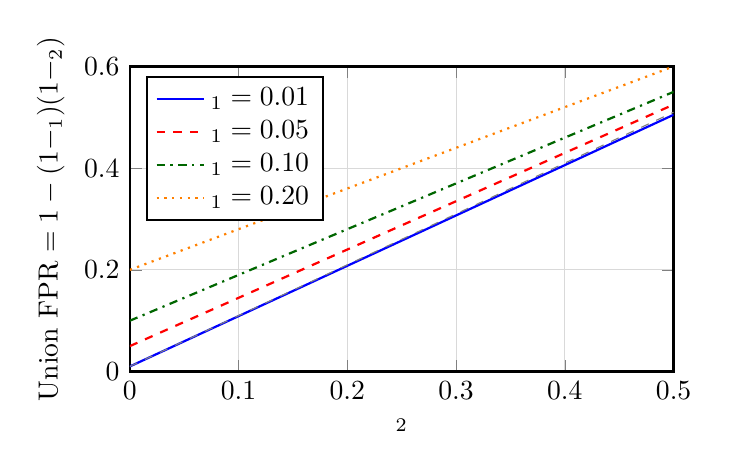
\begin{tikzpicture}
\begin{axis}[
	width=0.7\textwidth,
	height=0.45\textwidth,
	xlabel={$\fprate_2$},
	ylabel={Union FPR $= 1 - (1-\fprate_1)(1-\fprate_2)$},
	xmin=0, xmax=0.5,
	ymin=0, ymax=0.6,
	legend pos=north west,
	ymajorgrids, xmajorgrids,
	major grid style={gray!30},
	thick,
	samples=100,
	domain=0:0.5,
]
\addplot[blue, solid] {1-(1-0.01)*(1-x)};
\addlegendentry{$\fprate_1 = 0.01$}
\addplot[red, dashed] {1-(1-0.05)*(1-x)};
\addlegendentry{$\fprate_1 = 0.05$}
\addplot[black!60!green, dashdotted] {1-(1-0.10)*(1-x)};
\addlegendentry{$\fprate_1 = 0.10$}
\addplot[orange, dotted, thick] {1-(1-0.20)*(1-x)};
\addlegendentry{$\fprate_1 = 0.20$}
\addplot[gray, thin, dashed, forget plot] {x + 0.01};
\end{axis}
\end{tikzpicture}
\caption{Union false positive rate
$\fprate = 1 - (1-\fprate_1)(1-\fprate_2)$ as a function of $\fprate_2$
for several fixed values of $\fprate_1$.
The thin dashed gray line shows the additive approximation
$\fprate_1 + \fprate_2$ for $\fprate_1 = 0.01$;
for small rates, the union FPR is nearly additive, but the
product term $\fprate_1 \fprate_2$ becomes significant as rates grow.
By De Morgan duality, the intersection FNR has the same functional form
with $\fnrate_i$ replacing $\fprate_i$.}
\label{fig:union_fpr}
\end{figure}

\begin{example}[Numerical illustration of union error rates]
\label{ex:numerical_union}
Let $|U| = 1000$, $|A_1| = 100$, $|A_2| = 80$, and $|A_1 \cap A_2| = 30$.
Then $|A_1 \cup A_2| = 100 + 80 - 30 = 150$ and the partition weights for the union (\cref{eq:union_weights}) are
\begin{equation}
w_1 = \frac{70}{150} \approx 0.467, \quad
w_2 = \frac{50}{150} \approx 0.333, \quad
w_3 = \frac{30}{150} = 0.200.
\end{equation}
Suppose $\fprate_1 = 0.01$, $\fprate_2 = 0.02$, $\fnrate_1 = 0.05$, and $\fnrate_2 = 0.03$.
By \cref{thm:union_fprate}, the union FPR is
\begin{equation}
\fprate = 1 - (1 - 0.01)(1 - 0.02) = 1 - 0.99 \times 0.98 = 0.0298.
\end{equation}
By \cref{thm:union_fnrate}, the union FNR is
\begin{align}
\fnrate &\approx 0.467 \times 0.05 \times (1 - 0.02)
         + 0.333 \times 0.03 \times (1 - 0.01)
         + 0.200 \times 0.05 \times 0.03 \notag \\
       &\approx 0.02288 + 0.00990 + 0.00030 \approx 0.03307.
\end{align}
Thus $\tilde{A}_1 \cup \tilde{A}_2$ is a Bernoulli set approximating $A_1 \cup A_2$ with FPR $\approx 0.030$ and FNR $\approx 0.033$.
\end{example}

Several structural observations follow from the table.

The union and intersection formulas exhibit a duality:
the false positive rate of the union has the same functional form as the
false negative rate of the intersection, and vice versa.
This duality reflects De Morgan's laws: $A_1 \cup A_2 =
\SetComplement[\SetComplement[A_1] \cap \SetComplement[A_2]]$, so that
the union may be realized by complementing both operands, intersecting,
and complementing the result.
By \cref{thm:complement_rates}, each complementation exchanges the roles
of $\fprate$ and $\fnrate$, producing the observed symmetry.

\subsection{Closure properties}
\label{sec:closure}
The error rates in \cref{tab:set_ops} reveal that certain classes of
Bernoulli sets are closed under specific operations.

\begin{theorem}[Closure of positive Bernoulli sets under intersection]
\label{thm:closure_positive_intersect}
If $\tilde{A}_1$ and $\tilde{A}_2$ are positive Bernoulli sets, then
$\tilde{A}_1 \cap \tilde{A}_2$ is a positive Bernoulli set.
\end{theorem}
\begin{proof}
By \cref{cor:intersect_positive}, when $\fnrate_1 = \fnrate_2 = 0$,
the intersection has $\fnrate = 0$ and
$\fprate = w_1 \fprate_2 + w_2 \fprate_1
+ w_3 \fprate_1 \fprate_2 \geq 0$.
Since $\fnrate = 0$, the result is a positive Bernoulli set.
\end{proof}

\begin{theorem}[Closure of negative Bernoulli sets under union]
\label{thm:closure_negative_union}
If $\tilde{A}_1$ and $\tilde{A}_2$ are negative Bernoulli sets, then
$\tilde{A}_1 \cup \tilde{A}_2$ is a negative Bernoulli set.
\end{theorem}
\begin{proof}
By \cref{cor:union_negative}, when $\fprate_1 = \fprate_2 = 0$,
the union has $\fprate = 0$ and
$\fnrate = w_1 \fnrate_1 + w_2 \fnrate_2
+ w_3 \fnrate_1 \fnrate_2 \geq 0$.
Since $\fprate = 0$, the result is a negative Bernoulli set.
\end{proof}

\begin{remark}
Complement maps positive Bernoulli sets to negative Bernoulli sets and vice
versa by \cref{thm:complement_rates}.
In particular, the closure of positive sets under intersection and the
closure of negative sets under union are dual statements: applying
De Morgan's law and complementation converts one into the other.
\end{remark}

These closure properties constrain which expressions over Bernoulli sets
produce outputs that remain within the positive or negative class.
The following grammar characterizes the set-theoretic expressions that are
guaranteed to produce a positive Bernoulli set (production $\langle
\mathrm{exp} \rangle$) or a negative Bernoulli set (production $\langle
\mathrm{nexp} \rangle$):
\begin{align}
\label{eq:grammar_exp}
\langle \mathrm{exp} \rangle \; ::= \; &
    \langle \mathrm{aset} \rangle
    \;\mid\; \langle \mathrm{exp} \rangle \cup \langle \mathrm{exp} \rangle
    \;\mid\; \langle \mathrm{exp} \rangle \cap \langle \mathrm{exp} \rangle
    \;\mid\; \SetComplement[\langle \mathrm{nexp} \rangle] \\
\label{eq:grammar_nexp}
\langle \mathrm{nexp} \rangle \; ::= \; &
    \langle \mathrm{naset} \rangle
    \;\mid\; \langle \mathrm{nexp} \rangle \cup \langle \mathrm{nexp}
        \rangle
    \;\mid\; \langle \mathrm{nexp} \rangle \cap \langle \mathrm{nexp}
        \rangle
    \;\mid\; \SetComplement[\langle \mathrm{exp} \rangle]
\end{align}
where $\langle \mathrm{aset} \rangle$ denotes a positive Bernoulli set and
$\langle \mathrm{naset} \rangle$ denotes a negative Bernoulli set.

The grammar is justified as follows.
A union of positive Bernoulli sets is positive by
\cref{cor:union_positive}, and an intersection of positive sets is positive
by \cref{thm:closure_positive_intersect}; both productions are therefore included.
Since $A_1 \cap A_2 = \SetComplement[\SetComplement[A_1] \cup
\SetComplement[A_2]]$, the intersection of two positive sets may be
expressed as the complement of a union of two negative sets (via
\cref{thm:complement_rates}), which by
\cref{thm:closure_negative_union} is negative, and whose complement is
therefore positive.
The dual argument applies for the $\langle \mathrm{nexp} \rangle$
production.

\subsection{Asymptotic behavior of composed error rates}

The error-rate formulas above determine the \emph{expected} rates for composed approximate sets.
Within a region whose elements share one per-element error probability, the error count is binomial and the asymptotic normal approximation of~\cite{bernoulliSets} applies.
A marginal rate that averages several regions (for example the union false negative rate) has a Poisson-binomial count instead; its variance is the sum of the per-region binomial variances, which is at most the binomial variance at the marginal rate.

For example, the true negative rate of the union $\tilde{A}_1 \cup \tilde{A}_2$ has the asymptotic distribution
\begin{equation}
\TNR_\n \sim \normdist\!\left(\tnrate_1 \tnrate_2, \frac{\tnrate_1 \tnrate_2 (1-\tnrate_1 \tnrate_2)}{\n}\right),
\end{equation}
where $\n = u - |A_1 \cup A_2|$ is the number of negatives.
As $\n \to \infty$, the distribution converges in probability to $\tnrate_1 \tnrate_2$.

\begin{remark}[Convergence of intersections of positive approximate sets]
	Consider independent positive approximate sets
	$\PASet{A}[\fprate_1],\ldots,\PASet{A}[\fprate_k]$
	of the same objective set.
	As $k \to \infty$, $\bigcap_{i=1}^{k} \PASet{A}[\fprate_i]$ converges
	almost surely to $\Set{A}$, since each negative element survives with
	probability $\prod_{i=1}^{k} \fprate_i \to 0$.
	Dually, for negative approximate sets,
	$\bigcup_{i=1}^{k} \NASet{A}[\fnrate_i]$ converges almost surely
	to $\Set{A}$.
\end{remark}

\begin{remark}[Monoidal structure]
\label{rem:monoid}
The results above show that the collection of Bernoulli sets over $U$ is
closed under union and intersection (with computable output rates).
Since these operations inherit associativity and commutativity from the
powerset $2^U$, Bernoulli sets form a commutative semigroup under each.
If the degenerate-case axiom is adopted---$\Prob{\ASet{\EmptySet} =
\EmptySet} = 1$ and, dually, $\Prob{\ASet{U} = \Set{U}} = 1$ (see~\cite{bernoulliSets})---then $\EmptySet$ and $\Set{U}$ serve as
identity elements, yielding commutative monoids under union and
intersection respectively.
This is useful in practice: the $n$-ary union
$\bigcup_{i=1}^{n} \ASet{A}_i$ is precisely the monoidal fold, requiring only an
associative operation and an identity element.
The fold is exact for the realized sets and for the per-region rates.
Folding the marginal pairs of \cref{tab:set_ops} is exact only for the uniform rate (the false positive rate of a union fold, or the false negative rate of an intersection fold); the other marginal must be recomputed from the regions (see the remark on nested expressions above).
The operands must be distinct and independently constructed (\cref{asm:cross_set_indep}).
\end{remark}

%%%%%%%%%%%%%%%%%%%%%%%%%%%%%%%%%%%%
% Relational approximate sets
%%%%%%%%%%%%%%%%%%%%%%%%%%%%%%%%%%%%
\section{Relational probabilities}
\label{sec:relational}
The relational \emph{member-of} predicate $\in : U \times 2^U \to \{0,1\}$ is the set-indicator function, or the \emph{membership} predicate, which is true if $x$ is a member of the set $A$ and false otherwise.
By \cref{prop:element_rates}, given $x \in A$, $x \in \tilde{A}^\fprate_\tprate$ with probability $\tprate$ and given $x \notin A$, $x \in \tilde{A}^\fprate_\tprate$ with probability $\fprate$.
These probabilities are axiomatic in the second-order random approximate set model.

Other kinds of relational predicates are functions of the \emph{member-of} predicate, in particular the subset $\subseteq : 2^U \times 2^U \to \{0,1\}$, equality $= : 2^U \times 2^U \to \{0,1\}$, and
proper subset $\subset : 2^U \times 2^U \to \{0,1\}$ predicates respectively defined as (where $[\phi]$ denotes the Iverson bracket: $1$ if $\phi$ is true, $0$ otherwise)
\begin{align}
\label{def:subset_pred}
A \subseteq B	&= \prod_{x \in A} [x \in B],\\
\label{def:eq_pred}
A = B			&= (A\subseteq B) \land (B\subseteq A) \text{, and}\\
\label{def:proper_subset_pred}
A \subset B		&= (A \neq B) \land (A \subseteq B)
\end{align}
where complementary relations are naturally given by complements, e.g., $A \neq B = 1-(A = B)$.

\begin{theorem}
Given $X \subseteq Y$, $\tilde{X} \subseteq \tilde{Y}$ with probability
\begin{equation}
	\left(1 - \tprate_1\fnrate_2\right)^{|X|}
	\left(1 - \fprate_1\fnrate_2\right)^{|Y| - |X|}
	\left(1 - \fprate_1\tnrate_2\right)^{|U| - |Y|},
\end{equation}
where $\tilde{X}$ has a false positive rate $\fprate_1$ and a true positive rate $\tprate_1$ and $\tilde{Y}$ has a false positive rate $\fprate_2$ and true positive rate $\tprate_2$.
\end{theorem}
\begin{proof}
	$\tilde{X} \subseteq \tilde{Y}$ holds if and only if, for every element $j \in U$, $j \in \tilde{X}$ implies $j \in \tilde{Y}$.
	Equivalently, the event $j \in \tilde{X} \land j \notin \tilde{Y}$ must not occur for any $j$.
	By element-wise independence and cross-set independence (\cref{asm:cross_set_indep}), the probability is
	\begin{equation}
	\gamma = \prod_{j=1}^{u} \left(1 - \Prob{j \in \tilde{X}} \Prob{j \notin \tilde{Y}}\right),
	\end{equation}
	where the probabilities are conditioned on membership in $X$ and $Y$ respectively.
	Since $X \subseteq Y$, the universal set partitions into three blocks:
	\begin{enumerate}
		\item $X$: elements in both $X$ and $Y$ ($|X|$ elements),
		\item $Y \setminus X$: elements in $Y$ but not $X$ ($|Y| - |X|$ elements),
		\item $U \setminus Y$: elements in neither ($|U| - |Y|$ elements).
	\end{enumerate}
	Substituting the error rates for each block:
	\begin{itemize}
		\item Block 1: $\Prob{j \in \tilde{X}} = \tprate_1$ and $\Prob{j \notin \tilde{Y}} = \fnrate_2$.
		\item Block 2: $\Prob{j \in \tilde{X}} = \fprate_1$ and $\Prob{j \notin \tilde{Y}} = \fnrate_2$.
		\item Block 3: $\Prob{j \in \tilde{X}} = \fprate_1$ and $\Prob{j \notin \tilde{Y}} = \tnrate_2$.
	\end{itemize}
	Since each block contributes a constant factor per element, the product reduces to
	\begin{equation}
	\gamma =
	\left(1 - \tprate_1 \fnrate_2\right)^{|X|}
	\left(1 - \fprate_1 \fnrate_2\right)^{|Y| - |X|}
	\left(1 - \fprate_1 \tnrate_2\right)^{|U| - |Y|}.
	\qedhere
	\end{equation}
\end{proof}

\begin{corollary}
\label{cor:equality_prob}
Given $X = Y$, $\tilde{X}[\fprate_1][\tprate_1] = \tilde{Y}[\fprate_2][\tprate_2]$ with probability
\begin{equation}
\left(\tprate_1\tprate_2 + \fnrate_1\fnrate_2\right)^{|X|}
\left(\fprate_1\fprate_2 + \tnrate_1\tnrate_2\right)^{|U| - |X|}.
\end{equation}
\end{corollary}
\begin{proof}
$\tilde{X} = \tilde{Y}$ holds if and only if $\mathbf{1}_{\tilde{X}}(j) = \mathbf{1}_{\tilde{Y}}(j)$ for every $j \in U$.
By element-wise independence across elements, the probability is
$\prod_{j \in U} P(\mathbf{1}_{\tilde{X}}(j) = \mathbf{1}_{\tilde{Y}}(j))$.
Since $X = Y$, the universe partitions into two blocks:
\begin{itemize}
	\item $j \in X$: both indicators are independent Bernoulli trials with success probabilities $\tprate_1$ and $\tprate_2$ respectively, so they agree with probability $\tprate_1\tprate_2 + \fnrate_1\fnrate_2$.
	\item $j \notin X$: both indicators have success probabilities $\fprate_1$ and $\fprate_2$, so they agree with probability $\fprate_1\fprate_2 + \tnrate_1\tnrate_2$.
\end{itemize}
Since each block contributes a constant factor per element, the product reduces to the stated formula.
\end{proof}


\begin{corollary}
	Given $X = Y$, $\tilde{X}^\fprate_\tprate = \tilde{Y}^\fprate_\tprate$ with probability
	\begin{equation}
	\left(\tprate^2 + \fnrate^2\right)^{|X|}
	\left(\fprate^2 + \tnrate^2\right)^{|U| - |X|}.
	\end{equation}
\end{corollary}
\begin{proof}
Set $\fprate_1 = \fprate_2 = \fprate$ and $\tprate_1 = \tprate_2 = \tprate$
in the preceding corollary: the positive-block factor becomes
$\tprate^2 + \fnrate^2$ and the negative-block factor becomes
$\fprate^2 + \tnrate^2$.
\end{proof}


\begin{corollary}
	Given $X \subseteq Y$, if $\tilde{X}$ and $\tilde{Y}$ have no false positives ($\fprate_1 = \fprate_2 = 0$, that is, negative Bernoulli sets in the convention of \cref{sec:set_theory}), then $\tilde{X} \subseteq \tilde{Y}$ with probability
	\begin{equation}
	\left(1 - \tprate_1\fnrate_2\right)^{|X|}.
	\end{equation}
\end{corollary}
\begin{proof}
With $\fprate_1 = \fprate_2 = 0$, the
second and third factors of the subset theorem reduce to $1$ (each equals $1^n$).
Only the first factor remains.
Since $\fnrate_2 = 1 - \tprate_2$, this gives $(1 - \tprate_1 \fnrate_2)^{|X|}$.
Dually, for positive Bernoulli sets ($\fnrate_1 = \fnrate_2 = 0$) only the third factor remains, giving $(1 - \fprate_1 \tnrate_2)^{|U| - |Y|}$.
\end{proof}




\begin{corollary}
	Over an infinite universal set, the probability that two second-order random approximate sets realize the same value is $0$.
\end{corollary}
\begin{proof}
Each factor in the equality probability is strictly less than $1$
when $\fprate, \tprate \in (0,1)$. As $|U| \to \infty$, the product
of such factors raised to powers growing with $|U|$ tends to $0$.
\end{proof}

\begin{corollary}
	Over an infinite universal set, the probability that a second-order random approximate set realizes a value that is a subset of another realization of a second-order random approximate set is $0$.
\end{corollary}
\begin{proof}
The third factor of the subset probability,
$(1 - \fprate_1 \tnrate_2)^{|U|-|Y|}$, tends to $0$ as $|U| \to \infty$
whenever $\fprate_1 \tnrate_2 > 0$.
\end{proof}




%%%%%%%%%%%%%%%%%%%%%%%%%%%%%%%%
% Interval -- uncertainty
%%%%%%%%%%%%%%%%%%%%%%%%%%%%%%%%

\section{Interval arithmetic for uncertain rates}
\label{sec:intervals}
In practice, the expected false positive and true positive rates may not be known exactly.
This section develops an \emph{interval arithmetic} approach: each uncertain rate is represented by an interval guaranteed to contain the true value, and the error-rate formulas of \cref{sec:set_theory} are evaluated over these intervals to produce guaranteed bounds on the output rates.

\begin{definition}
An interval is a convex set of real numbers.
We denote by $\Interval{\underbar{x},\bar{x}}$ an interval with a lower-bound $\underbar{x}$ and an upper-bound $\bar{x}$.
\end{definition}

A confidence interval may be specified in interval notation.
Here, however, we consider an algebra for interval arithmetic and put it to use quantifying our ignorance about the distribution of parameters after, for instance, a union operation.

The error-rate formulas of \cref{sec:set_theory} depend upon the false positive and false negative rates being \emph{known}.
Any parameters that are not known with certainty may be replaced by intervals that (are assumed to) contain the true value.
As a consequence, the output error rate will also be an interval.

\emph{Maximum} uncertainty is when the parameter value is in the interval $[0,1]$, e.g., $[\fprate] = [0,1]$, and \emph{minimum} uncertainty is when the parameter is some value in the degenerate interval $[x,x]$, e.g., $[\fprate] = [.2,.2]$. The more certain---the smaller the width of the intervals---the more certain the output rate.

When using interval arithmetic, the \emph{dependency problem} can lead to overly pessimistic bounds.
In our case, the formulae are simple enough to ensure dependencies are satisfied. The following example illustrates the approach for the union false positive rate.

\begin{example}
	Suppose two approximate sets have false positive rates known only to lie in $[\fprate_1]$ and $[\fprate_2]$ respectively.
	The union FPR formula (\cref{thm:union_fprate}) is $\fprate = 1 - (1-\fprate_1)(1-\fprate_2)$, which is monotonically increasing in both $\fprate_1$ and $\fprate_2$.
	Evaluating at the endpoints yields guaranteed bounds:
	\begin{equation}
		[\fprate] = \bigl[1 - (1 - \underline{\fprate}_1)(1 - \underline{\fprate}_2),\;
		             1 - (1 - \overline{\fprate}_1)(1 - \overline{\fprate}_2)\bigr].
	\end{equation}
	For instance, if $[\fprate_1] = [0.01, 0.05]$ and $[\fprate_2] = [0.02, 0.08]$, then $[\fprate] = [0.0298, 0.126]$.
\end{example}

We may not be interested in the \emph{expected} value, but the smallest set of values such that with probability $1-\gamma$ the true rate
realizes some value in the set, which is typically an \emph{interval}, i.e., a confidence interval.

Intervals represent an uncertainty and they manifest themselves in two independent ways.
The common notion of the \emph{confidence interval} is a product of the probabilistic model, i.e., the realized true positive rate $\tprateob$, which is normally centered around the expected true positive rate $\tprate$ as discussed in~\cite{bernoulliSets}.
We may use \emph{interval arithmetic} and replace point values with interval values, point values being a degenerate case.
Basic interval arithmetic is presented in~\cite{basicinterval}; the foundational treatment is due to Moore~\cite{mooreInterval}.

A set sampled from $\tilde{A}[\fprate][\tprate]$ is an approximate set such that the $\gamma\cdot 100\%$ asymptotic confidence intervals for the realized false negative and false positive rates are respectively given by
\begin{equation}
\Interval{\fnrate} = \fnrate \pm \sqrt{\frac{\fnrate(1-\fnrate)}{p}}\, \Phi^{-1}\!\left(\frac{1+\gamma}{2}\right)
\end{equation}
and
\begin{equation}
\Interval{\fprate} = \fprate \pm \sqrt{\frac{\fprate(1-\fprate)}{n}}\, \Phi^{-1}\!\left(\frac{1+\gamma}{2}\right),
\end{equation}
where $p$ and $n$ are the number of positives and negatives respectively and $\Phi^{-1}$ is the inverse CDF of the standard normal (see \cref{eq:conf_fpr,eq:conf_tpr}).

\subsection{Interval propagation through set operations}

The simple error-rate formulas---union FPR, intersection FNR, and complement---are monotonically increasing in each input rate.
The weighted formulas (union FNR, intersection FPR, and set difference rates) have \emph{mixed monotonicity}: they increase in same-type rates ($\fnrate$ in $\fnrate$, $\fprate$ in $\fprate$) and decrease in cross-type rates ($\fnrate$ in $\fprate$, $\fprate$ in $\fnrate$).
Replacing point-valued rates with intervals and evaluating at the appropriate endpoints for each variable yields guaranteed bounds on the output rates, for known partition weights; when the weights are also uncertain, each weighted rate is linear in the weights and its extremes lie at vertices of the weight simplex.

\begin{theorem}[Complement]
\label{thm:uncertain_rates_comp_set}
The \emph{complement} of an approximate set with a false negative rate $\Interval{\fnrate}$ and false positive rate $\Interval{\fprate}$ is an approximate set with a false negative rate $\Interval{\fprate}$ and false positive rate $\Interval{\fnrate}$.
\end{theorem}
\begin{proof}
Follows immediately from \cref{thm:complement_rates}: complementation swaps positives and negatives, so it swaps the false positive and false negative rates. Since the interval endpoints swap accordingly, the result holds.
\end{proof}

\begin{theorem}[Union]
\label{thm:uncertain_rates_union}
Given two approximate sets with interval-valued rates $[\fprate_1]$, $[\fnrate_1]$ and $[\fprate_2]$, $[\fnrate_2]$, the union has interval-valued false positive rate
\begin{equation}
[\fprate] = \bigl[1 - (1 - \underline{\fprate}_1)(1 - \underline{\fprate}_2),\;
             1 - (1 - \overline{\fprate}_1)(1 - \overline{\fprate}_2)\bigr],
\end{equation}
since the union FPR formula $\fprate = 1 - (1-\fprate_1)(1-\fprate_2)$ from \cref{thm:union_fprate} is monotonically increasing in both $\fprate_1$ and $\fprate_2$.
Since the union FNR (\cref{eq:union_fnr}) increases in $\fnrate_1, \fnrate_2$ and decreases in $\fprate_1, \fprate_2$, the upper bound is attained at $(\overline{\fnrate}_1, \overline{\fnrate}_2, \underline{\fprate}_1, \underline{\fprate}_2)$ and the lower bound at $(\underline{\fnrate}_1, \underline{\fnrate}_2, \overline{\fprate}_1, \overline{\fprate}_2)$.
\end{theorem}

\begin{remark}
Intersection and set difference follow analogously: the intersection FNR has the same form as the union FPR (by the De Morgan duality noted in \cref{sec:set_ops_summary}), and the set difference is handled by substituting complemented intervals per \cref{thm:uncertain_rates_comp_set}.
\end{remark}




%%%%%%%%%%%%%%%%%%%%%%%%%%%%%%%%%
% Conclusion
%%%%%%%%%%%%%%%%%%%%%%%%%%%%%%%%%

\section{Conclusion}
\label{sec:conclusion}

Under cross-set independence, complement, union, intersection, and set difference of Bernoulli sets yield (possibly higher-order) Bernoulli sets whose per-region error probabilities are closed-form functions of the operand rates, and whose marginal rates are cardinality-weighted averages of them.
These are the standard independent-OR and independent-AND rules~\cite{broderMitzenmacher2004,parker1975,dalvi2007}, collected here in one notation.
At the level of realized sets, union and intersection form commutative monoids with the empty set and universal set as identities.
Relational predicates---subset and equality---admit exact probability formulas that factorize element-wise.
An interval arithmetic extension propagates uncertain rate parameters through set operations, yielding guaranteed bounds when parameters are only approximately known.

\paragraph{Practical implications.}
For a system built on independently constructed Bloom filters, the formulas of \cref{sec:set_theory} give the error rates of any set-theoretic expression, provided they are applied region by region: the per-element probability of each intermediate result must be tracked by the membership pattern of the element in all operands (see the remark on nested expressions in \cref{sec:set_ops_summary}).
Reusing the marginal (FPR, FNR) pair of an intermediate result in a further operation is not valid in general, and confidence intervals for marginal rates must account for the Poisson-binomial error count.

\paragraph{Open problems.}
The partition weights $w_1, w_2, w_3$ in the set-operation formulas require knowledge of the objective set cardinalities, which are typically unknown (\cref{rem:unknown_partitions}).
Developing principled estimators for these cardinalities from the approximate sets themselves, with quantified bias and variance, is a natural next step.

\paragraph{Companion papers.}
The Bernoulli set model, including the axioms, error-count distributions, asymptotic limits, confidence intervals, and higher-order composition theorem, is developed in~\cite{bernoulliSets}.
The probability distributions of binary classification measures (positive predictive value, negative predictive value, accuracy, Youden's $J$) are derived in~\cite{bernoulliMeasures}.
The joint entropy of error counts and the information-theoretic space complexity lower bound are developed in~\cite{bernoulliEntropy}.


\bibliography{references}

\end{document}
